\documentclass[a4paper]{article}

\usepackage{tecnico_relatorio}

\usepackage{textcomp}
\usepackage[hypcap]{caption} % makes \ref point to top of figures and tables
%\usepackage{rotating}
\usepackage{float}
\usepackage[nottoc]{tocbibind}
\usepackage[utf8]{inputenc}
\usepackage{graphicx}
\usepackage[justification=centering]{caption}
\usepackage{listings}
\usepackage{indentfirst} % indent first paragraph in section
\usepackage{geometry}	% margins

\begin{document}
	\newgeometry{left=4.5cm,right=4.5cm}

	\trSetImage{img/tecnico_logo}{6cm} % Logotipo do Técnico
    
    \trSetCourse{Mestrado em Engenharia Electrotécnica \\e de Computadores}
    
	\trSetSubject{Sistemas Computacionais Embebidos}
	
	\trSetType{2ª Parte}

	\trSetTitle{Sistema de Monitorização e Alarme}

	\trSetBoxStyle{0.3}

	\trSetGroupNo{Grupo 6}

	\trSetAuthorNr{3}

	\trSetAuthors
	{
		\begin{center}
			Gonçalo Ribeiro

			73294
		\end{center}
	}{
		\begin{center}
			Francisco Leal

			72939
		\end{center}
	}{
		\begin{center}
			Ricardo Amendoeira

			73373
		\end{center}
	}

	\trSetProfessor{Prof. Carlos Almeida}

\trMakeCover
    
	\restoregeometry

	\tableofcontents
	\pagenumbering{gobble}

	\pagebreak

	\pagenumbering{arabic}
	\setcounter{page}{1}



	\section{Introdução}
    
    Neste trabalho pretende-se controlar o sistema criado na primeira parte deste projecto, via série, utilizando um sistema remoto, com várias \textit{threads}, que corre o sistema operativo eCos.
    

	\section{Esquema de Comunicações}


	\begin{figure}[h]
    	\centering
    	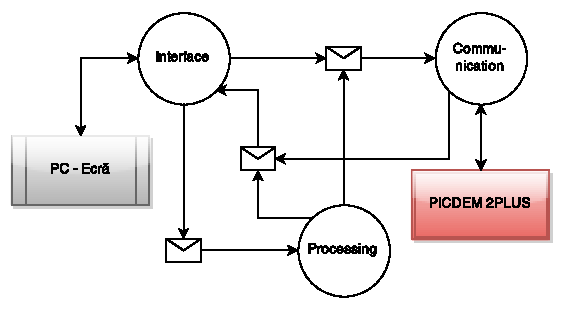
\includegraphics[scale=1]{img/threads}
        \caption{Interligação entre os vários blocos do sistema}
        \label{fig:threads_communication}
	\end{figure}




	\section{Estruturas de Dados}
    Na segunda parte do trabalho foi adicionado um \textit{buffer} circular de modo a gerir a memória partilhada entre as várias \textit{threads} do programa. Para a gerir foi adicionado um \textit{mutex} para garantir que o acesso a esta zona critica de memória é restringido a uma \textit{thread} de cada vez apenas.
    
	Para além de esta zona crítica existe também a zona crítica de acesso ao ecrã. Para tal, foi criado um \textit{mutex} que salvaguarda o acesso ao ecrã para dispor informação ao utilizador.
    
    De modo a sincronizar as \textit{threads} e possibilitar a comunicação entre estas são usadas duas \textit{mailboxes} que permite o acesso às \textit{threads} de processamento e de comunicação. Não é necessário criar uma \textit{mailbox} para a \textit{thread} de interface com o utilizador visto que esta só tem que aceder directamente à memória partilhada.




	\section{Blocos Principais}
    
    A utilização de \textit{threads} permite uma segmentação do código que dificilmente se consegue utilizando métodos mais regulares de programação. Assim, utilizando esta vantagem é possível subdividir o programa nos seguintes blocos de funcionamento.

	\subsection{Interface}
    
    Para a interface é usada uma \textit{thread} que tem como funções:
	
    \begin{itemize}
      \item receber comandos do utilizador
      \item enviar e receber informação para as outras \textit{threads} via \textit{mailboxes}
      \item imprimir resultados no ecrã
    \end{itemize}

	Este bloco permite a interacção do utilizador com o \textit{eCos} e com a placa, libertando assim a complexidade do processamento e comunicação entre os vários componentes. A principal responsabilidade desta \textit{thread} é distribuir os pedidos do utilizador pelos vários componentes responsáveis pelas restantes funções do sistema operativo.


	\subsection{Processamento}

	O processamento recebe na \textit{mailbox} os comandos designados para esta \textit{thread}, identificando a função pedida. Esta lida com os acessos à memoria partilhada, tal como monitorização de forma periódica de transferência de registos do PIC para o eCos.



	\subsection{Comunicação}

	A comunicação com a placa de desenvolvimento é feita via porta RS-232, usando um protocolo série. Cada transferência corresponde a 1 byte e são usados apenas os pinos TX, RX e GND. O protocolo série é bidireccional usando um pino para cada direcção (TX de \textit{master} para \textit{slave} e RX de \textit{slave} para \textit{master}). Em estado \textit{idle}, cada pino de comunicação está a \textit{high} e é levado a \textit{low} durante o período de um símbolo, para indicar o início da transferência. Nos oito períodos seguintes são enviados os oito bits a transmitir, terminando a transmissão com o pino a voltar a \textit{high}.
    
    Do lado do \textit{eCos} a comunicação tem o principal objectivo da manutenção e actualização do \textit{buffer} circular traduzindo a informação recebida pela placa para a memória partilhada pelas várias \textit{threads}, disponibilizando a informação ao sistema operativo.
    
    
    
    \section{Placa de Desenvolvimento}

	Para implementar a segunda parte do projecto foi necessário desactivar o modo de \textit{sleep} do sistema, para não serem perdidos símbolos da comunicação. Na verdade bastava ter uma interrupção que acordasse o microcontrolador com periodicidade inferior ao período da \textit{baud rate} usada.
    
    A comunicação utiliza a interface de USART do PIC, que é constituída por um registo que gera uma interrupção quando há dados novos para ler e/ou quando há dados para transmitir. A leitura de mensagens da RS-232 é feita através de um interrupção que lê o novo byte recebido na USART, que é colocado num \textit{buffer}. A posição do \textit{buffer} onde os bytes recebidos são colocados é controlada por uma máquina de estados simples que verifica os bytes de início e fim das mensagens (\texttt{SOM} e \texttt{EOM}). A escrita para o \textit{master} é feita através de \textit{polling}.
    
    
    

	\section{Conclusão}

    O trabalho feito na segunda parte do projecto permite potencialmente criar redes de sensores que são controladas por um único computador central que corre eCos. Foram implementadas funcionalidades que permitem: activar alarmes, consultar valores dos sensores e consultar registos sobre esses alarmes, entre outros.
    
    O uso de \textit{threads} neste trabalho, embora lúdico, é de pouca utilidade prática para as funcionalidades implementadas, o que tornou o sistema mais complexo e mais propício a erros, o que é de evitar em contexto não académico.
    
    Num sistema de produção seria preferível usar um método de comunicação mais actual e prático, como USB ou até um sistema sem fios. No entanto, sabemos por experiência própria\footnote{\url{http://hackerschool.io/portfolio/talus/}}  que estes tipos de comunicação podem não ser os mais simples de aprender, o que justifica a utilização de comunicação série no projecto.
    
    O projecto podia ter sido levado a um grau superior de desenvolvimento, não fosse o facto de o acesso às ferramentas necessárias ser bastante limitado e o desenvolvimento do \textit{software} ser dificultado devido à utilização de três sistemas operativos em simultâneo.

	O projecto foi útil para nos introduzir ao conceito de sistemas operativos em tempo real, os quais podem ser úteis em vários ramos da industria, por exemplo aeroespacial ou indústria de fabrico.
    

\end{document}